\documentclass[conference]{IEEEtran}

\usepackage[T1]{fontenc}
\usepackage{amsmath}
\usepackage{amssymb}
\usepackage{graphicx}
\usepackage{booktabs}
\usepackage{microtype}
\usepackage{url}
\usepackage[backend=biber, style=numeric-comp, sorting=none, giveninits=true,
    maxbibnames=6, url=false, doi=true, eprint=true, isbn=false]{biblatex}
\addbibresource{references.bib}
\AtBeginBibliography{\footnotesize}

\begin{document}

\title{Selective Underwater Image Enhancement\\for Object Detection with YOLO11}

\author{
    \IEEEauthorblockN{1\textsuperscript{st} Nguyen Quoc Bao}
    \IEEEauthorblockA{
        \textit{The University of Danang}\\
        \textit{University of Science and Technology}\\
        Da Nang, Vietnam\\
        102250412@hv.dut.udn.vn
    }
    \and
    \IEEEauthorblockN{2\textsuperscript{nd} Phan Le Van Minh}
    \IEEEauthorblockA{
        \textit{The University of Danang}\\
        \textit{University of Science and Technology}\\
        Da Nang, Vietnam\\
        102250417@hv.dut.udn.vn
    }
}

\maketitle

\begin{abstract}
    Underwater image enhancement (UIE) is often applied before object detection, and recent studies report that using one enhancement method for every image does not raise detection accuracy. We look at a selective alternative on the RUOD benchmark with a YOLO11n detector. A small ResNet18 selector picks, for each image, the raw version, SCNet, or Semi-UIR. Its training labels come from an out-of-fold procedure, so no detector scores an image it was trained on. The selector reaches the accuracy of raw images and leaves most images unchanged. We also add a control in which the oracle chooses between a raw image and its horizontal flip. The control gives a gain similar to that of oracles over enhanced versions, so part of the oracle gap may come from changes in detector output between slightly different inputs. Fusing the predictions of four views with weighted boxes fusion gives a small gain over raw images. Finally, a detector trained on raw and enhanced versions of the training images scores higher on raw test images than a detector trained on raw images only, although it also sees more images during training. In our experiments, enhancement was more useful as training data than as a per-image choice at test time.
\end{abstract}

\begin{IEEEkeywords}
    underwater image enhancement, underwater object detection, selective enhancement, YOLO11, RUOD, UIEB
\end{IEEEkeywords}

% ---------------------------------------------------------------------------
\section{Introduction}
\label{sec:intro}

Cameras on autonomous underwater vehicles (AUVs) and remotely operated vehicles (ROVs) record images that suffer from light absorption and scattering, both of which depend on wavelength~\cite{fuRethinkingGeneralUnderwater2023,liUnderwaterImageEnhancement2019}. Red light fades at shallow depth. The images that result tend to show a green or blue cast, low contrast, soft edges, and haze.

Deep learning models for underwater image enhancement (UIE), such as SCNet~\cite{fuUnderwaterImageEnhancement2022} and Semi-UIR~\cite{huangContrastiveSemisupervisedLearning2023}, report high PSNR and SSIM against reference images. It is common to place such a model in front of a detector as a preprocessing step, on the assumption that a cleaner image is easier to detect objects in.

Awad et al.~\cite{awadRevisitingUnderwaterImage2026} report that this assumption does not always hold. In their study, applying one enhancer to all images often lowered detection accuracy compared with the raw images, although some images did improve. On RUOD~\cite{fuRethinkingGeneralUnderwater2023} they also computed a mixed-set upper bound, in which each image takes the best of ten versions (the raw image and nine enhanced versions), chosen with ground-truth annotations. This oracle raised the mean per-image mAP from 0.68 to 0.77 (+0.09).

That upper bound leaves two practical questions, and we examine both here. First, can the choice between versions be made from the raw image alone, without annotations? Second, how much of an oracle gain can be traced to the enhancement itself, and how much to differences in detector output between versions of the same image?

\begin{figure}[t]
    \centering
    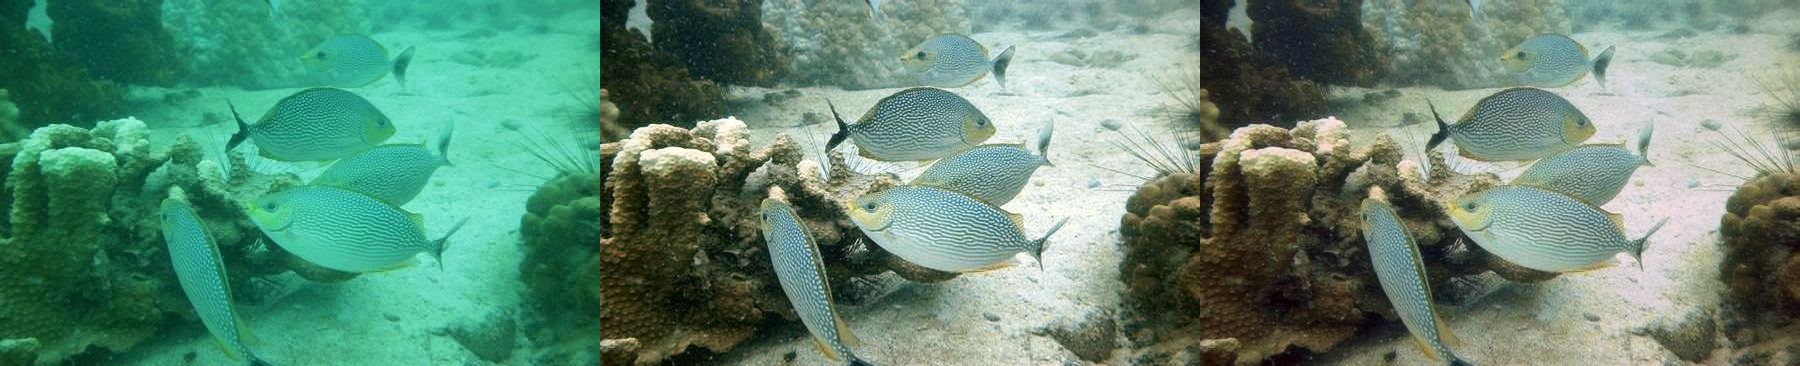
\includegraphics[width=\columnwidth]{figures/sample_enhancement.png}
    \caption{Sample RUOD image before and after enhancement. From left to right: raw input (orig), Semi-UIR~\cite{huangContrastiveSemisupervisedLearning2023}, and SCNet~\cite{fuUnderwaterImageEnhancement2022}.}
    \label{fig:sample}
\end{figure}

We study these questions with YOLO11n~\cite{jocherUltralyticsYOLO2024} on the 14{,}000-image RUOD benchmark. The candidate versions of each image are the raw image, SCNet, and Semi-UIR. Our results are as follows.
\begin{itemize}
    \item We build a selection pipeline whose selector labels come from a three-fold out-of-fold detector protocol with a margin of $\delta = 0.01$. A ResNet18 selector~\cite{heDeepResidualLearning2015} (7.7\,ms per image) looks only at the raw image resized to $224 \times 224$.
    \item On the 4{,}200 test images, the selector with a decision threshold reaches 0.6159 mAP@0.5:0.95 (+3.2\% of the oracle gap closed), against 0.6155 for raw images. It keeps the raw image for 85.5\% of inputs. Applying SCNet to every image gives 0.6129, Semi-UIR gives 0.6084, and random choice gives 0.6120.
    \item In a control experiment, an oracle that chooses between the raw image and its horizontal flip, with no enhancement involved, gains +0.0207 per-image mAP. This is 144\% of the +0.0144 gained by the oracle over raw and SCNet.
    \item Fusing the predictions of four views with weighted boxes fusion (WBF)~\cite{solovyevWeightedBoxesFusion2021} gives +0.0023 mAP@0.5:0.95 on the full set. The 95\% confidence interval of the per-image difference, $[+0.0014, +0.0051]$, lies above zero.
    \item A detector trained on all three versions of the training images raises raw-image mAP@0.5:0.95 from 0.6037 to 0.6210 (+0.018) compared with a detector trained on raw images only.
\end{itemize}

% ---------------------------------------------------------------------------
\section{Related Work}
\label{sec:related}

\subsection{Underwater Image Enhancement}

SCNet~\cite{fuUnderwaterImageEnhancement2022} is built to handle different water types. At several scales of a U-Net, it decorrelates spatial activations with instance whitening and standardizes the channel mean and variance, so the learned features depend less on the water type.

Semi-UIR~\cite{huangContrastiveSemisupervisedLearning2023} addresses the lack of paired training data with a mean-teacher setup and contrastive regularization. A reliable bank holds pseudo-labels ranked by a no-reference image quality score. At inference time, an attention-guided illumination modulation network (AIMnet) works from an estimated multi-scale Gaussian luminance map.

Both models were evaluated on UIEB~\cite{liUnderwaterImageEnhancement2019} with PSNR and SSIM. These metrics compare an output with a reference image. They do not measure detection.

\subsection{Enhancement for Underwater Object Detection}

Fu et al.~\cite{fuRethinkingGeneralUnderwater2023} released RUOD for underwater detection and noted that common enhancement methods had inconsistent effects across detector families. Luo et al.~\cite{luoMASYOLOv11ImprovedUnderwater2025} proposed MAS-YOLOv11, which adds multi-scale attention heads for cluttered underwater scenes. Huang et al.~\cite{huangAMIEODAdaptiveMultiExperts2026} proposed AMIEOD, which selects among experts for low-illumination images.

Awad et al.~\cite{awadRevisitingUnderwaterImage2026} compared nine enhancers with several modern detectors. No enhancer beat the raw images on the whole test set, and the authors defined the per-image mixed-set upper bound described in Section~\ref{sec:intro}. That bound needs ground-truth annotations at test time, and it uses a separately trained detector for each version.

\subsection{Box Fusion and Test-Time Augmentation}

Test-time augmentation combines the predictions made on transformed copies of an input. Non-maximum suppression (NMS) keeps one box from each group of overlapping boxes and drops the rest. Weighted boxes fusion (WBF)~\cite{solovyevWeightedBoxesFusion2021} instead clusters the overlapping boxes from all views and averages their coordinates, weighted by confidence.

% ---------------------------------------------------------------------------
\section{Methodology}
\label{sec:method}

\subsection{System Overview}

Let $x \in \mathbb{R}^{H \times W \times 3}$ be an underwater RGB image. We use two enhancers with fixed weights released by their authors: SCNet ($E_{\mathrm{SC}}$) and Semi-UIR ($E_{\mathrm{SU}}$). The candidate versions are
\begin{equation}
    \mathcal{V}(x) = \{\, v_0, v_1, v_2 \,\} = \{\, x,\; E_{\mathrm{SC}}(x),\; E_{\mathrm{SU}}(x) \,\}.
\end{equation}
A selector $f_\theta$ looks at the raw image $x$ and predicts an index $\hat{k} \in \{0, 1, 2\}$. The chosen version $v_{\hat{k}}$ is then passed to a fine-tuned YOLO11n detector $D$.

\subsection{Enhancers and Processing Pipeline}
\label{sec:method-enh}

Both enhancers run at the native resolution ($640$\,px long edge) with the released weights and no fine-tuning.
\begin{itemize}
    \item \textbf{SCNet:} We keep only the enhancement decoder branch and drop the VGG16 network that serves as a perceptual loss during training. The input is reflect-padded to a multiple of 8. The output is cropped back and quantized to $[0, 255]$.
    \item \textbf{Semi-UIR:} The luminance map $L(x)$ is estimated by convolving the luminance channel with Gaussian kernels at $\sigma \in \{15, 60, 90\}$, averaging the logarithmic responses, and normalizing to $[0, 255]$. The input and the luminance map are reflect-padded to a multiple of 16. One image takes about 2\,s.
\end{itemize}
Enhanced images are saved as JPEG ($\text{quality} = 95$) and share the bounding box labels of the raw images.

\subsection{Out-of-Fold (OOF) Selector Labeling}
\label{sec:method-labels}

A detector that has trained on an image tends to score it too well, which would distort the selector labels. We therefore use a three-fold out-of-fold protocol.
\begin{enumerate}
    \item The 9{,}800 RUOD training images are split into three folds $\mathcal{F}_0, \mathcal{F}_1, \mathcal{F}_2$ with random seed 0 (MD5 hash: \texttt{ea44b385539c}).
    \item For each fold $k \in \{0, 1, 2\}$, a YOLO11n detector is trained for 30 epochs with AdamW on all three versions of the other two folds ($\approx 19{,}600$ images).
    \item The final checkpoint (\texttt{last.pt}) predicts on all three versions of the held-out fold $\mathcal{F}_k$ ($\text{conf} = 0.001$, $\text{IoU} = 0.7$).
    \item \texttt{pycocotools} gives the per-image mAP@0.5:0.95 values $m_{i,0}, m_{i,1}, m_{i,2}$. Images without annotations get 0.
\end{enumerate}
With a margin $\delta = 0.01$, the target label of image $i$ is
\begin{equation}
    y_i =
    \begin{cases}
        0                    & \text{if } \max_{k \in \{1, 2\}} m_{i,k} - m_{i,0} < \delta, \\
        \arg\max_{k} m_{i,k} & \text{otherwise}.
    \end{cases}
\end{equation}

\subsection{Selector Architecture and Decision Rules}

The selector is a ResNet18~\cite{heDeepResidualLearning2015} pretrained on ImageNet, with a linear head of three outputs. Its input is the raw image resized to $224 \times 224 \times 3$. One image takes 7.7\,ms on an NVIDIA Tesla T4 GPU. We train it in two ways.
\begin{itemize}
    \item \textbf{Class-weighted cross-entropy (\texttt{ce}):}
          \begin{equation}
              \mathcal{L}_{\mathrm{ce}} = -\sum_{c=0}^2 w_c \cdot \mathbb{I}(y = c) \log p_c,
          \end{equation}
          where $w_c$ is the inverse class frequency.
    \item \textbf{mAP regression (\texttt{reg}):} the network predicts the three mAP values $(\hat{m}_0, \hat{m}_1, \hat{m}_2)$ with a Smooth L1 loss.
\end{itemize}

\subsubsection{Decision Threshold ($\tau$)}
To limit enhancement calls on images that do not benefit, we take $k^* = \arg\max_{k \in \{1, 2\}} p_k$ only if $p_{k^*} - p_0 > \tau$. Otherwise the raw image is kept. For regression the condition is $\hat{m}_{k^*} - \hat{m}_0 > \tau$.

\subsubsection{Validation Selection Criterion}
Always choosing the raw image already gives 58.2\% accuracy on the training labels and 62.4\% on the test labels, so accuracy is a poor guide. We select models and thresholds by chosen-mAP on a held-out 20\% validation split (1{,}960 images):
\begin{equation}
    \text{chosen-mAP} = \frac{1}{N_{\mathrm{val}}} \sum_{i=1}^{N_{\mathrm{val}}} m_{i, \hat{y}_i}.
\end{equation}
The thresholds chosen this way are $\tau = 0.625$ for \texttt{ce} and $\tau = 0.040$ for \texttt{reg}.

\subsection{Evaluation by Composing Saved Predictions}

The evaluation on the 4{,}200 RUOD test images has four parts.
\begin{enumerate}
    \item A single detector (\texttt{full.pt}) is trained for 50 epochs on all three versions of the 9{,}800 training images ($29{,}400$ images in total, 10{,}732\,s of training).
    \item Test predictions for each version are computed once and stored. A policy is scored by composing the stored predictions of the version it picks for each image and running \texttt{pycocotools}.
    \item We resample the per-image mAP differences against the raw baseline 1{,}000 times (paired bootstrap). This gives 95\% confidence intervals and bootstrap p-values $p_{\text{boot}}(\Delta \le 0)$.
    \item The share of the oracle gap that a policy closes is
          \begin{equation}
              G = \frac{\mathrm{mAP}_{\mathrm{policy}} - \mathrm{mAP}_{\mathrm{orig}}}{\mathrm{mAP}_{\mathrm{oracle}} - \mathrm{mAP}_{\mathrm{orig}}} \times 100\%.
          \end{equation}
\end{enumerate}

\subsection{Oracle Control with Horizontal Flip}
\label{sec:method-noise}

To see how much of an oracle gain depends on enhancement, we add a control based on a horizontal flip $T_{\mathrm{flip}}$. For an input $x$, the predictions $D(T_{\mathrm{flip}}(x))$ are mapped back to the coordinates of the original image with $T_{\mathrm{flip}}^{-1}(\hat{\mathcal{B}})$. The flipped image has the same colors and contrast as $x$. Any difference between $m_{i, \mathrm{orig}}$ and $m_{i, \mathrm{flip}}$ therefore comes from how the detector responds to the position of the content, including the effect of NMS. We define
\begin{equation}
    \text{Oracle}_{\{\mathrm{orig}, \mathrm{flip}\}}(i) = \max \left( m_{i, \mathrm{orig}},\; m_{i, \mathrm{flip}} \right).
\end{equation}
If this oracle gains about as much as $\text{Oracle}_{\{\mathrm{orig}, E(x)\}}$, we read it as a sign that part of the oracle gain comes from variation in detector output and not from the enhancement.

\subsection{Multi-View Weighted Boxes Fusion}
\label{sec:method-wbf}

We fuse the boxes predicted on the raw, flipped, SCNet, and Semi-UIR views with WBF~\cite{solovyevWeightedBoxesFusion2021}. The settings are fixed: $\text{IoU}_{\mathrm{thr}} = 0.6$, $\text{skip\_box\_thr} = 0.001$, and at most 150 boxes per view.

% ---------------------------------------------------------------------------
\section{Experimental Setup}
\label{sec:setup}

\subsection{Datasets}

\textbf{UIEB}~\cite{liUnderwaterImageEnhancement2019} has 890 paired real underwater images. We use its standard 90-image test set at native resolution to check that the two enhancers reproduce the published numbers.

\textbf{RUOD}~\cite{fuRethinkingGeneralUnderwater2023} has 14{,}000 underwater images (9{,}800 train, 4{,}200 test) in 10 categories: \emph{holothurian, echinus, scallop, starfish, fish, corals, diver, cuttlefish, turtle, jellyfish}. We resize the long edge to 640\,px.

\subsection{Implementation Details}

Experiments ran on Kaggle with two NVIDIA Tesla T4 GPUs, PyTorch 2.11 (CUDA 12.8), and Ultralytics 8.4.174. YOLO11n used $640 \times 640$ input, the AdamW optimizer, batch size 32, and seed 0. ResNet18 was trained for 15 epochs with AdamW (learning rate $3 \times 10^{-4}$, weight decay $10^{-2}$) on an 80/20 split of the training set (7{,}840 train, 1{,}960 val).

\subsection{Metrics}

PSNR and SSIM come from \texttt{scikit-image}. Detection accuracy is COCO mAP@0.5 and mAP@0.5:0.95 from \texttt{pycocotools}. Confidence intervals (CI) are paired bootstrap 95\% intervals over 1{,}000 resamples.

% ---------------------------------------------------------------------------
\section{Results and Discussion}
\label{sec:results}

\subsection{Enhancer Check on UIEB}
\label{sec:res-uieb}

Table~\ref{tab:uieb} compares our measurements on the 90-image UIEB test split with the published numbers. Our PSNR for SCNet is within 0.35\,dB of the published value, and for Semi-UIR within 0.38\,dB. SSIM differs by less than 0.02. Both enhancers raise PSNR by more than 4.5\,dB over the raw inputs.

\begin{table}[t]
    \centering
    \caption{PSNR and SSIM on UIEB test set (90 images, mean $\pm$ std).}
    \label{tab:uieb}
    \setlength{\tabcolsep}{4pt}
    \begin{tabular}{l c c c c}
        \toprule
                                                                   & \multicolumn{2}{c}{Ours}  & \multicolumn{2}{c}{Published}                  \\
        Method                                                     & PSNR (dB)                 & SSIM                          & PSNR  & SSIM   \\
        \midrule
        Raw input                                                  & $17.90 \pm 5.35$          & $0.776 \pm 0.137$             & --    & --     \\
        SCNet~\cite{fuUnderwaterImageEnhancement2022}              & $22.43 \pm 4.43$          & $0.879 \pm 0.082$             & 22.08 & 0.8625 \\
        Semi-UIR~\cite{huangContrastiveSemisupervisedLearning2023} & $\mathbf{24.21} \pm 4.03$ & $\mathbf{0.886} \pm 0.069$    & 24.59 & 0.9010 \\
        \midrule
        Per-image oracle$^{\dagger}$                               & 24.95                     & 0.9010                        & --    & --     \\
        \bottomrule
        \multicolumn{5}{l}{\footnotesize $^{\dagger}$Best of the three versions per image, chosen per metric.}
    \end{tabular}
\end{table}

\begin{table}[t]
    \centering
    \caption{Number of UIEB test images (out of 90) winning per metric.}
    \label{tab:best}
    \begin{tabular}{l c c c}
        \toprule
        Metric & Raw input & SCNet & Semi-UIR \\
        \midrule
        PSNR   & 6         & 24    & 60       \\
        SSIM   & 10        & 29    & 51       \\
        \bottomrule
    \end{tabular}
\end{table}

No single version wins on every image (Table~\ref{tab:best}). By PSNR, Semi-UIR is best on 60 images, SCNet on 24, and the raw input on 6. The per-image oracle reaches 24.95\,dB, which is 0.74\,dB above Semi-UIR alone. On image 703 the raw PSNR is 40.63\,dB, while SCNet and Semi-UIR give 27.54\,dB and 26.38\,dB. Image 713 goes the other way: the raw PSNR is 9.75\,dB, and the two enhancers reach 19.64\,dB and 28.54\,dB.

\subsection{Out-of-Fold Labels on the RUOD Training Set}
\label{sec:res-oof}

The three-fold procedure on the 9{,}800 training images gave 5{,}704 raw labels (58.2\%), 2{,}208 SCNet labels (22.5\%), and 1{,}888 Semi-UIR labels (19.3\%).

On these out-of-fold predictions, raw images reach 0.5808 mAP@0.5:0.95 (0.6873 per image). Uniform SCNet gives 0.5785 (0.6859 per image) and uniform Semi-UIR gives 0.5729 (0.6817 per image). The out-of-fold oracle reaches 0.7164 per-image mAP, which is 0.0291 above raw.

\subsection{Detection Results on the RUOD Test Set}
\label{sec:res-detection}

Table~\ref{tab:ruod} lists every policy on the 4{,}200 test images, all scored with the same detector.

\begin{table*}[t]
    \centering
    \caption{Object detection performance on the RUOD test set (4{,}200 images) with YOLO11n.}
    \label{tab:ruod}
    \resizebox{\textwidth}{!}{
        \begin{tabular}{l c c c c c c c}
            \toprule
            Policy                               & mAP@0.5         & mAP@0.5:0.95    & Per-image mAP   & Gap Closed (All / Per)   & $\Delta$ vs. Raw [95\% CI]          & $p_{\text{boot}}(\Delta \le 0)$ & Selection (Orig / SC / Semi) \\
            \midrule
            Always Raw (\texttt{orig})           & 0.8468          & 0.6155          & 0.7186          & 0.0\% / 0.0\%            & -- (Baseline)                       & 1.000                           & 4200 / 0 / 0                 \\
            Always SCNet                         & 0.8449          & 0.6129          & 0.7154          & -18.1\% / -13.6\%        & -0.0031 [-0.0049; -0.0013]          & 1.000                           & 0 / 4200 / 0                 \\
            Always Semi-UIR                      & 0.8422          & 0.6084          & 0.7130          & -50.0\% / -24.2\%        & -0.0056 [-0.0077; -0.0034]          & 1.000                           & 0 / 0 / 4200                 \\
            Random Selection                     & 0.8444          & 0.6120          & 0.7148          & -24.7\% / -16.3\%        & -0.0038 [-0.0054; -0.0021]          & 1.000                           & 1387 / 1401 / 1412           \\
            \midrule
            Selector \texttt{ce}                 & 0.8472          & 0.6146          & 0.7173          & -6.4\% / -5.4\%          & -0.0012 [-0.0025; 0.0000]           & 0.970                           & 2210 / 1101 / 889            \\
            \textbf{Selector \texttt{ce+$\tau$}} & \textbf{0.8474} & \textbf{0.6159} & 0.7182          & \textbf{+3.2\%} / -1.5\% & \textbf{-0.0004 [-0.0010; +0.0003]} & 0.851                           & \textbf{3593 / 319 / 288}    \\
            Selector \texttt{reg}                & 0.8457          & 0.6142          & 0.7182          & -8.8\% / -1.7\%          & -0.0004 [-0.0018; +0.0009]          & 0.734                           & 2133 / 1373 / 694            \\
            Selector \texttt{reg+$\tau$}         & 0.8462          & 0.6146          & 0.7183          & -5.9\% / -1.4\%          & -0.0003 [-0.0014; +0.0008]          & 0.745                           & 3019 / 828 / 353             \\
            \midrule
            Oracle (Upper Bound)                 & \textbf{0.8524} & \textbf{0.6296} & \textbf{0.7417} & 100.0\% / 100.0\%        & +0.0231 [+0.0216; +0.0247]          & 0.000                           & 2620 / 846 / 734             \\
            \bottomrule
        \end{tabular}
    }
\end{table*}

\begin{table}[t]
    \centering
    \caption{Validation performance on 1{,}960 held-out images and test confusion matrix of Selector \texttt{ce+$\tau$} on 4{,}200 test images.}
    \label{tab:confusion}
    \resizebox{\columnwidth}{!}{
        \begin{tabular}{l c c c c}
            \toprule
            \multicolumn{5}{c}{\textbf{A. Validation Split Performance (1{,}960 images)}}                                                 \\
            Variant                     & $\tau$                    & Chosen-mAP          & \multicolumn{2}{c}{Gap Closed}                \\
            \midrule
            Always Raw                  & --                        & 0.6924              & \multicolumn{2}{c}{0.0\%}                     \\
            \texttt{ce}                 & 0                         & 0.6923              & \multicolumn{2}{c}{-0.4\%}                    \\
            \textbf{\texttt{ce+$\tau$}} & \textbf{0.625}            & \textbf{0.6931}     & \multicolumn{2}{c}{\textbf{+2.5\%}}           \\
            \texttt{reg}                & 0                         & 0.6918              & \multicolumn{2}{c}{-2.4\%}                    \\
            \texttt{reg+$\tau$}         & 0.040                     & 0.6931              & \multicolumn{2}{c}{+2.2\%}                    \\
            Oracle                      & --                        & 0.7202              & \multicolumn{2}{c}{100.0\%}                   \\
            \midrule
            \multicolumn{5}{c}{\textbf{B. Test Confusion Matrix (Rows: True Oracle, Columns: Pred.)}}                                     \\
            Oracle Label                & Pred. Raw                 & Pred. SCNet         & Pred. Semi-UIR                      & Total   \\
            \midrule
            Raw (\texttt{orig})         & \textbf{2{,}259} (86.2\%) & 176 (6.7\%)         & 185 (7.1\%)                         & 2{,}620 \\
            SCNet                       & 708 (83.7\%)              & \textbf{83} (9.8\%) & 55 (6.5\%)                          & 846     \\
            Semi-UIR                    & 626 (85.3\%)              & 60 (8.2\%)          & \textbf{48} (6.5\%)                 & 734     \\
            \midrule
            Total Predicted             & 3{,}593 (85.5\%)          & 319 (7.6\%)         & 288 (6.9\%)                         & 4{,}200 \\
            \bottomrule
        \end{tabular}
    }
\end{table}

\begin{table}[t]
    \centering
    \caption{Per-class AP@0.5:0.95 across input policies on RUOD test set.}
    \label{tab:perclass}
    \resizebox{\columnwidth}{!}{
        \begin{tabular}{l c c c c c}
            \toprule
            Class       & Raw             & SCNet           & Semi-UIR        & Selector \texttt{ce+$\tau$} & Oracle          \\
            \midrule
            holothurian & 0.4966          & 0.4910          & 0.4877          & 0.4966                      & 0.5102          \\
            echinus     & 0.5305          & 0.5250          & 0.5187          & 0.5298                      & 0.5446          \\
            scallop     & 0.4957          & 0.4941          & 0.4791          & 0.4958                      & 0.5058          \\
            starfish    & 0.5508          & 0.5409          & 0.5431          & 0.5506                      & 0.5652          \\
            fish        & 0.5198          & 0.5196          & 0.5181          & 0.5191                      & 0.5337          \\
            corals      & 0.5386          & 0.5367          & 0.5338          & 0.5377                      & 0.5519          \\
            diver       & 0.7456          & 0.7467          & 0.7397          & 0.7462                      & 0.7638          \\
            cuttlefish  & 0.8360          & 0.8320          & 0.8315          & 0.8361                      & 0.8487          \\
            turtle      & 0.8383          & 0.8390          & 0.8330          & 0.8384                      & 0.8518          \\
            jellyfish   & 0.6026          & 0.6041          & 0.5991          & \textbf{0.6089}             & 0.6208          \\
            \midrule
            Mean        & \textbf{0.6155} & \textbf{0.6129} & \textbf{0.6084} & \textbf{0.6159}             & \textbf{0.6296} \\
            \bottomrule
        \end{tabular}
    }
\end{table}

\subsubsection{Uniform Enhancement}
Applying SCNet to every image lowers mAP@0.5:0.95 by 0.0026 ($-0.0031$ per image, CI $[-0.0049; -0.0013]$). Semi-UIR lowers it by 0.0071 ($-0.0056$ per image, CI $[-0.0077; -0.0034]$). Both intervals lie below zero ($p_{\text{boot}} = 1.000$). Random selection also lowers accuracy, by 0.0038 per image.

\subsubsection{Selector Accuracy}
The two selectors without a threshold (\texttt{ce} and \texttt{reg}) lose a little accuracy, which is consistent with enhancement being called on images that do not benefit. With the threshold, Selector \texttt{ce+$\tau$} reaches 0.6159 mAP@0.5:0.95 (+3.2\% of the gap closed), close to the 0.6155 of raw images. The 95\% CI of the per-image difference, $[-0.0010; +0.0003]$, includes zero ($p_{\text{boot}} = 0.851$).

\subsubsection{Confusion Matrix}
Table~\ref{tab:confusion} gives the validation scores and the test confusion matrix. Overall accuracy on the test set is 56.9\%, below the 62.4\% that always choosing the raw image would give. SCNet improved mAP on 846 test images, and the selector chose SCNet for 83 of them (9.8\%). Semi-UIR improved mAP on 734 images, and the selector chose it for 48 (6.5\%).

The selector stays near the raw baseline mostly because the threshold $\tau = 0.625$ leaves the raw image in place for 85.5\% of the inputs (3{,}593 images). Its cost is 7.7\,ms per image.

\subsubsection{Per-Class Results}
Table~\ref{tab:perclass} lists AP for each of the 10 classes. On \emph{holothurian}, \emph{echinus}, and \emph{scallop} the selector stays close to the raw baseline. Its largest difference is on \emph{jellyfish} (0.6089 against 0.6026). That is one class, we did not compute a confidence interval for it, and we have not tested what causes it.

\subsection{Oracle Gain With and Without Enhancement}
\label{sec:res-noise}

Table~\ref{tab:noise} lists oracles over several candidate sets on the 4{,}200 test images.

\begin{table}[t]
    \centering
    \caption{Oracle comparison between optical enhancers and horizontal reflection on RUOD test set.}
    \label{tab:noise}
    \resizebox{\columnwidth}{!}{
        \begin{tabular}{l c c c c}
            \toprule
            Oracle Candidate Set                                   & Size & mAP@0.5:0.95 & $\Delta$ Per-Image [95\% CI] & Non-Raw \% \\
            \midrule
            $\{\text{orig}, \text{orig rerun}\}$                   & 2    & 0.6159       & +0.0005 [+0.0003; +0.0006]   & 2.3\%      \\
            $\{\text{orig}, \text{scnet}\}$                        & 2    & 0.6250       & +0.0144 [+0.0133; +0.0154]   & 31.6\%     \\
            $\{\text{orig}, \text{semiuir}\}$                      & 2    & 0.6250       & +0.0164 [+0.0150; +0.0179]   & 31.7\%     \\
            $\{\text{orig}, \text{flip}\}$ (control)               & 2    & 0.6300       & +0.0207 [+0.0193; +0.0221]   & 38.5\%     \\
            \midrule
            UIE oracle (orig, SCNet, Semi-UIR)                     & 3    & 0.6300       & +0.0234 [+0.0219; +0.0250]   & 44.2\%     \\
            $\{\text{orig}, \text{flip}, \text{SC}, \text{Semi}\}$ & 4    & 0.6386       & +0.0353 [+0.0336; +0.0371]   & 58.6\%     \\
            \bottomrule
        \end{tabular}
    }
\end{table}

The oracle over the raw image and its flipped copy reaches 0.6300 mAP@0.5:0.95, the same as the three-version oracle over raw, SCNet, and Semi-UIR. Per image, the flip oracle gains +0.0207, which is 144\% of the gain for SCNet (+0.0144). The three-version oracle is higher per image (+0.0234). The flipped copy has gone through no enhancement, so its gain reflects only how the detector responds to a mirrored input.

With four candidates (raw, flip, SCNet, Semi-UIR) the oracle reaches 0.6386. The expected maximum of several random variables does not decrease as variables are added. A larger candidate set therefore raises the oracle whether or not the added candidates carry useful information.

The selector labels come from the same out-of-fold scores. The correlation between the flip gain and the SCNet gain is 0.306. If a large share of each label reflects variation in detector output, a classifier that sees only pixels has little to learn from, which agrees with the selector results above. We ran this control with one detector only, so the size of the effect may differ for other detectors.

\subsection{Fusion and Confidence-Based Selection}
\label{sec:res-fusion}

Table~\ref{tab:fusion} lists methods that need no ground-truth labels at test time.

\begin{table}[t]
    \centering
    \caption{Multi-view fusion and confidence selection on RUOD test set.}
    \label{tab:fusion}
    \resizebox{\columnwidth}{!}{
        \begin{tabular}{l c c c}
            \toprule
            Method                             & mAP@0.5:0.95    & $\Delta$ Full    & $\Delta$ Per-Image [95\% CI]        \\
            \midrule
            Raw Baseline                       & 0.6155          & --               & --                                  \\
            WBF(orig, flip)                    & 0.6145          & -0.0009          & -0.0002 [-0.0019; +0.0014]          \\
            WBF(orig, SCNet)                   & 0.6085          & -0.0070          & -0.0050 [-0.0065; -0.0035]          \\
            WBF(orig, SCNet, Semi-UIR)         & 0.6111          & -0.0044          & -0.0025 [-0.0044; -0.0007]          \\
            \textbf{WBF(orig, flip, SC, Semi)} & \textbf{0.6177} & \textbf{+0.0023} & \textbf{+0.0032 [+0.0014; +0.0051]} \\
            \midrule
            Confidence \texttt{conf\_top5}     & 0.6129          & -0.0025          & -0.0021 [-0.0035; -0.0006]          \\
            Confidence \texttt{conf\_sum}      & 0.6136          & -0.0018          & -0.0018 [-0.0034; -0.0003]          \\
            \bottomrule
        \end{tabular}
    }
\end{table}

\subsubsection{Selection by Confidence}
Choosing the version by detector confidence (\texttt{conf\_top5} or \texttt{conf\_sum}) lowered accuracy by 0.0025 and 0.0018 mAP. Enhancement may raise the confidence of false positives in the background, but we did not test this.

\subsubsection{Four-View WBF}
WBF over two views, or over raw, SCNet, and Semi-UIR, did not beat raw images. WBF over four views (raw, flip, SCNet, Semi-UIR) reaches 0.6177 mAP@0.5:0.95, a gain of +0.0023 on the full set and +0.0032 per image. The 95\% CI of the per-image gain, $[+0.0014; +0.0051]$, lies above zero. Among the test-time methods we tried, it is the only one with such an interval. It needs four detector passes and both enhancers for every image.

\subsection{Training the Detector on Several Versions}
\label{sec:res-domains}

We also looked at the use of enhanced images during training. Table~\ref{tab:detector_comparison} compares a detector trained on raw images only with the final detector trained on all three versions, both scored on raw test images with the Ultralytics validator.

\begin{table}[t]
    \centering
    \caption{Comparison of YOLO11n baseline (trained on raw only) and multi-version detector evaluated on raw test images (Ultralytics validator).}
    \label{tab:detector_comparison}
    \resizebox{\columnwidth}{!}{
        \begin{tabular}{l c c c c}
            \toprule
            Detector Model                 & Training Data                         & Epochs      & mAP@0.5          & mAP@0.5:0.95     \\
            \midrule
            YOLO11n Baseline (Raw)         & 9{,}800 raw images                    & 50          & 0.8446           & 0.6037           \\
            \textbf{YOLO11n Multi-Version} & \textbf{29{,}400 images (3 versions)} & \textbf{50} & \textbf{0.8540}  & \textbf{0.6210}  \\
            \midrule
            Difference ($\Delta$)          & +19{,}600 enhanced images             & --          & \textbf{+0.0094} & \textbf{+0.0173} \\
            \bottomrule
        \end{tabular}
    }
\end{table}

Training on raw, SCNet, and Semi-UIR images for 50 epochs did not hurt detection on raw images. mAP@0.5:0.95 rose from 0.6037 to 0.6210 (+0.0173) and mAP@0.5 from 0.8446 to 0.8540. For the multi-version detector, per-class mAP@0.5:0.95 is 0.501 for \emph{holothurian}, 0.532 for \emph{echinus}, 0.501 for \emph{scallop}, 0.555 for \emph{starfish}, 0.527 for \emph{fish}, 0.552 for \emph{corals}, 0.751 for \emph{diver}, 0.842 for \emph{cuttlefish}, 0.843 for \emph{turtle}, and 0.608 for \emph{jellyfish}.

The multi-version detector sees three times as many images per epoch as the raw-only detector. This comparison therefore does not separate the effect of image diversity from the effect of more training data. In our experiments, enhancement was more useful as training data than as a per-image choice at test time.

% ---------------------------------------------------------------------------
\section{Conclusion}
\label{sec:conclusion}

We tested selective underwater image enhancement for object detection with YOLO11n on RUOD. In this setting we found the following.

Applying SCNet or Semi-UIR to every image lowered mAP@0.5:0.95 by 0.0026 and 0.0071 compared with raw inputs. A ResNet18 selector (7.7\,ms per image) with a threshold of $\tau = 0.625$ matched the raw baseline (0.6159 against 0.6155, +3.2\% of the gap closed), mostly because it kept the raw image for 85.5\% of inputs.

An oracle over the raw image and its horizontal flip gained +0.0207 per-image mAP, which is 144\% of the SCNet oracle gain of +0.0144. This suggests that part of the oracle gap comes from variation in detector output between inputs, and a selector working from pixels would have little to learn from it. Choosing a version by detector confidence lowered mAP by up to 0.0025. Four-view WBF gave +0.0023 on the full set, with a per-image 95\% CI of $[+0.0014, +0.0051]$.

Training on all three versions of the images raised raw-image mAP@0.5:0.95 from 0.6037 to 0.6210 (+0.0173) over raw-only training, though the multi-version detector also saw more images. All results come from one detector, one dataset, and one training run per configuration. Other detectors and other datasets are the next step.

\printbibliography

\end{document}